\section{Simulations}
\label{sec:simulation}

Prior to the start of operations, the main purpose of Mu2e simulation was to verify the expected performance of the experiment and to allow optimization of the detector design. That required an accurate, detailed, and flexible model of the experiment. In the analysis phase, the simulation will be used to optimize alignment, calibration, and reconstruction algorithms, to estimate the expected detector acceptance and resolution, and to develop analysis algorithms. The Mu2e simulation was designed to satisfy both of these objectives.

The Mu2e simulation is based on the Geant4 framework~\cite{geant4:2003,geant4:2006,geant4:2016}, including a description of the {\em as built} geometry and the material composition for both the sub-system parts and the experimental hall; the temporal and spatial structure of the proton beam; magnetic field maps; the implementation of the detector response as measured at beam tests and with cosmic rays; and a complete interface with the calibration database. A set of custom event generators dedicated to the conversion electron channel and the main sources of background are also used, and full events are simulated with overlapping beam background particles. Additional studies have been performed using other Monte Carlo codes (MARS\cite{MARS:2009}, MCNP\cite{MARS:2009, MCNP:2012}, FLUKA\cite{FLUKA:2013}, PHITS\cite{PHITS:2018}) to validate Geant4 predictions and to estimate their uncertainty.

The following sections describe the simulation workflow, the detector modeling, the physics generators, and the production campaigns in more detail.


\subsection{Simulation workflow}
The simulation of the large number of events expected in Mu2e requires some optimization of the processing time. This is achieved with a staged simulation approach together with resampling techniques. Given the statistical nature of the particle interactions in the material crossed before reaching the detectors, it's possible, where appropriate, to reuse many times the particles stored at the end of one stage ({\em resampling}) increasing the available statistics at a reduced cost of CPU time. The absence of statistical biases ({\em oversampling}) must be checked case by case. The staged approach helps to save additional CPU time when no changes occur in the first stages and it's sufficient to rerun only the last stages. In addition, different particle range cuts can be used in each stage to avoid unnecessary particle tracing. 

The main beam simulation is divided into four stages:
\begin{enumerate}
\item from the 8 GeV proton beam on the Production Target (PT) to the entrance of the Detector Solenoid (DS);
\item from DS entrance to the stopping target;
\item from the stopping target to the exit from the DS volume (tracker, calorimeter, and cosmic ray veto hits are stored);
\item detector response and digitization.
\end{enumerate}

The initial beam protons are given the nominal beam energy and direction, distributed across the PS entrance as a symmetric Gaussian with the width expected from beam simulations. The time of each proton is sampled from a distribution generated by detailed simulations of the slow extraction and active extinction system. To save processing time, charged particles that exit the PS volume forward are killed.

Special workflows have been developed to optimize the production of dedicated samples as well. Pion decay can be disabled to increase the number of stopped pions in the stopping target, and the stopped pion probability is then corrected for the pion survival probability depending on its lifetime. The first stage of the antiproton simulation has also been divided into four phases to use a customized differential cross section for antiproton production and optimize the absorber window located at the center of TS. The cosmic ray simulation requires a dedicated workflow as well. In the first stage secondaries produced by the CRY generator~\cite{CRY:2007} according to the flux at sea level are traced from the top of the Mu2e building to the DS. Events are divided into three categories according to the energy deposited in the Cosmic Ray Veto (CRV): high (E>16 MeV), low (E<16 MeV), or null (neutrons or particles passing through the TS hole). In the following stage, particles are resampled and traced through the detector. Finally, digitization is performed. In all cases, only the events with a minimum energy deposit in the tracker, the calorimeter, or the cosmic ray veto are passed to the digitization stage.


\subsection{Event generators}
A set of generators has been realized to have a more accurate simulation of the particle yield from the stopping target. Starting from the position and time of the stopped muons or pions, the following single particles can be generated with isotropic direction: conversion electron (Leading Log spectrum~\cite{Czarnecki:2011mx, Szafron:2017guu}), conversion positron (Leading Log spectrum~\cite{Czarnecki:2011mx, Szafron:2017guu} rescaled to the expected peak momentum of 92.3 MeV/c), DIO (Leading Log spectrum~\cite{Szafron:2016}), muon capture secondaries (protons and deuterons spectrum adapted from Ref.~\cite{TWIST:2020, ALCAP:2022}, neutron spectrum adapted from Ca measurements~\cite{MCnspectrum:1978} and normalized according to Ref.~\cite{MCnnorm:1965}, x-rays and gamma rays used to study the Stopping Monitor response are generated as single lines), radiative muon capture secondaries (photon spectrum from the fit of experimental data~\cite{TRIUMF:1999} with the closure approximation~\cite{closureapprox}), radiative pion capture secondaries (photon spectrum adapted from Mg data ~\cite{Bistirlich:1972}). Cosmic ray studies are performed with the CRY generator to evaluate the cosmic background and the CORSIKA generator~\cite{CORSIKA:1998} to estimate the uncertainty on flux normalization. A custom generator to produce antiprotons from protons interaction in the production target has been developed fitting the existing data and extrapolating them to the 8 GeV Mu2e beam energy~\cite{Mu2e:2022ggl}.

\subsection{Pileup simulation}
In addition to simulating particles of interest for physics studies and calibration, Mu2e must model the pileup of the many low energy particles produced by beam particles and decay/capture products of the vast majority of stopped muons which do not convert to electrons, or produce a particle which could be a signal background. Pileup is not itself a source of background for physics analyses, but the detector signals it generates can significantly affect the reconstruction efficiency and/or resolution of signal-like particles.

Mu2e simulates pileup using Geant-4, starting with protons hitting the production target (POT), as described above. Charged particles traveling backward and entering the TS are check-pointed as they enter the DS. Neutral particles that exit the beamline are check-pointed as they exit the TS or PS volume.

In subsequent simulation jobs, each check-pointed particle's passage through the DS is resampled 1000 to 10000 times, depending on the sample. Particles producing energy deposits in the detector sensitive volumes are saved, along with their genealogy and energy deposits. To allow correct normalization when used downstream, the fraction of saved events is calculated automatically during the resampling, relative to the original number of simulated POT, and stored in the conditions database.

Resampled muons stopping in the stopping target are check-pointed before they decay and then resampled 10000 times in turn to model pileup from muon capture and decay daughters. The muon lifetime is randomly sampled for each resampling, and custom codes are used to randomly select a decay mode. These same check-pointed target-stopped muons are also used as starting space points in the signal generators described above. The efficiency of resampled stopped muons producing energy deposits in sensitive volumes is computed and recorded in the database. 
The breakdown of signals expected from simulated pileup by time and stream in individual Mu2e detector sensor elements (straws for tracker, etc.) is shown in Fig.~\ref{fig:sim_pileup}.

\begin{figure}[ht!]
\centering
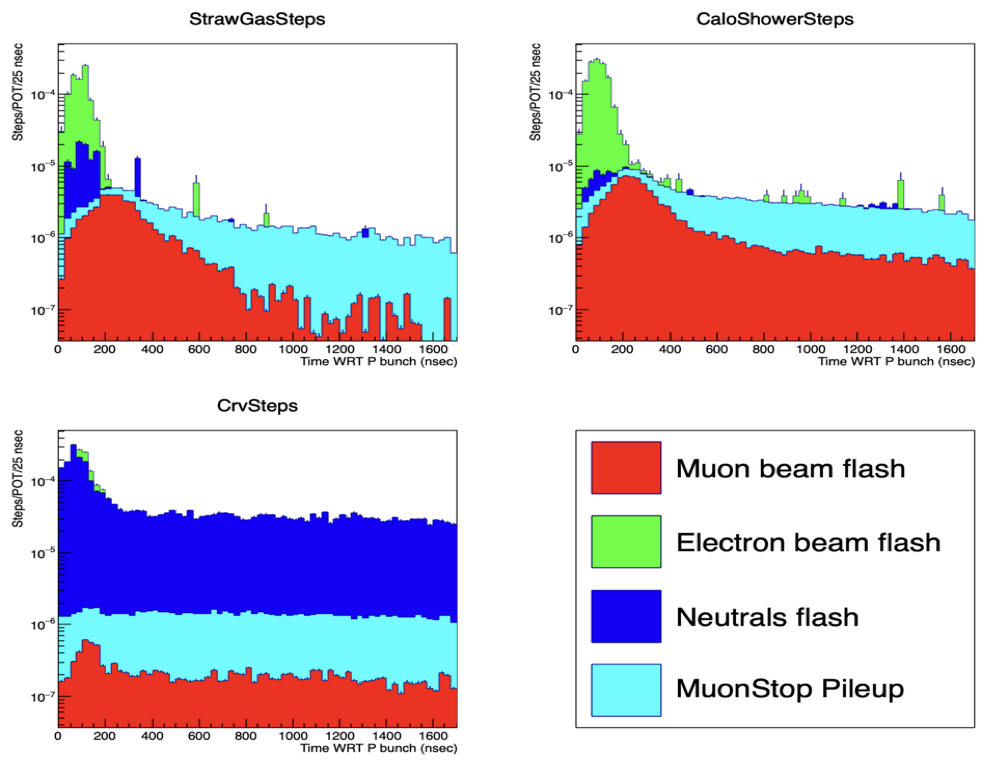
\includegraphics[width=0.8\textwidth]{figures/sim_pileup.png}%
\caption{Simulated signal counts in individual detector elements per POT relative to the arrival time of protons on the production target, wrapped to the beam pulse period, for the four pileup streams described in the text.}
\label{fig:sim_pileup}
\end{figure}

Pileup in the CRV is dominated by the neutral particles (mostly neutrons) leaving the PS. As the cross-section for generating signals in the CRV is small, these can be resampled many times, currently 10000. A physics list including detailed neutron interactions is used for this stage. Neutral CRV pileup resampling dominates the resources needed for pileup simulation, as the required statistics are large and the processes involved are time-consuming to model.

Pileup is overlaid on signal events by adding the sensitive volume energy deposits from an appropriate number of pileup daughters to the energy deposits generated by the signal process particle. Pileup data are read through art secondary input streams, in sequential mode, starting from a random starting event.
The number of pileup daughters needed is computed for each event by sampling the expected POT distribution, scaling that by the products of the relevant resampling efficiencies read from the database, and then applying Poisson fluctuations. The resulting summed energy deposits are then passed through the detector response simulation. Since the proton pulse intensity is expected to be relatively constant over millisecond timescales, and the pulse trains are long, the time of each pileup particle energy deposit is wrapped around the 1695 ns bunch period when summing.

Most Mu2e pileup simulations use a POT intensity distribution modeled by a log-normal distribution with Spill Duty Factor (SDF) = 60\%~\cite{Mu2e:2022ggl}, scaled to the average beam intensity expected for operations with either 1 or 2 booster batches. A time sequence of POT computed using a detailed beam extraction simulation can also be used.
The workflow for pileup simulation from POT and subsequent mixing onto simulated signals is shown in Fig.~\ref{fig:dts_mixing}.

Even when leveraged by resampling, simulating pileup from POT is very inefficient. Using $\sim7M$  core-hours of processing time, the most recent simulation campaign produced roughly 5 seconds (1.3 seconds) of experiment running time (beam live time). These samples also show statistical artifacts due to over-sampling of some particles. To avoid these limitations, Mu2e is developing code to overlay pileup extracted from beam data on simulated signals. By triggering randomly, Mu2e can record essentially unlimited pileup events with essentially zero resource cost that will naturally track the real POT intensity, and follow changing detector conditions. Unlike simulated signals and pileup, which are merged prior to digitization, pileup from beam data will be already digitized. Digital pileup that don't overlap with simulated signal particle energy deposits in time or channel can be merged trivially. Digital pileup that overlaps in both time and channel with simulated signals will be handled by dedicated codes. For the tracker, at the expected nominal beam intensity with 1 booster batch, 98\% of pileup signals are non-overlapping. 

The event identity of mixed (digital) pileup plus simulated (signal) events is given by the simulated event, to allow digitized pileup frames to be reused, and to distinguish them as Monte Carlo. Most conditions data used in simulating the signal and reconstructing the combined event are keyed to the pileup. This includes dead or noisy channels, sensor and electronics response, and resolutions. For effects which are not simulated, such as individual straw miss-alignments, conditions data are taken from the simulation. Preliminary studies overlaying digitized simulated pileup on simulated conversion electrons, using a very naive overlap resolution algorithm, shows nearly identical results post reconstruction as energy deposit pileup overlay. Digital pileup overlay is currently only implemented for the tracker. Extension of the digital pileup overlay algorithms to include the calorimeter and CRV, and development of more sophisticated algorithms for treating overlapping signals, as planned for the immediate future. The workflow for mixing pileup from random triggers onto simulated signals is shown in Fig.~\ref{fig:dig_mixing}.

\begin{figure}[ht!]
\centering
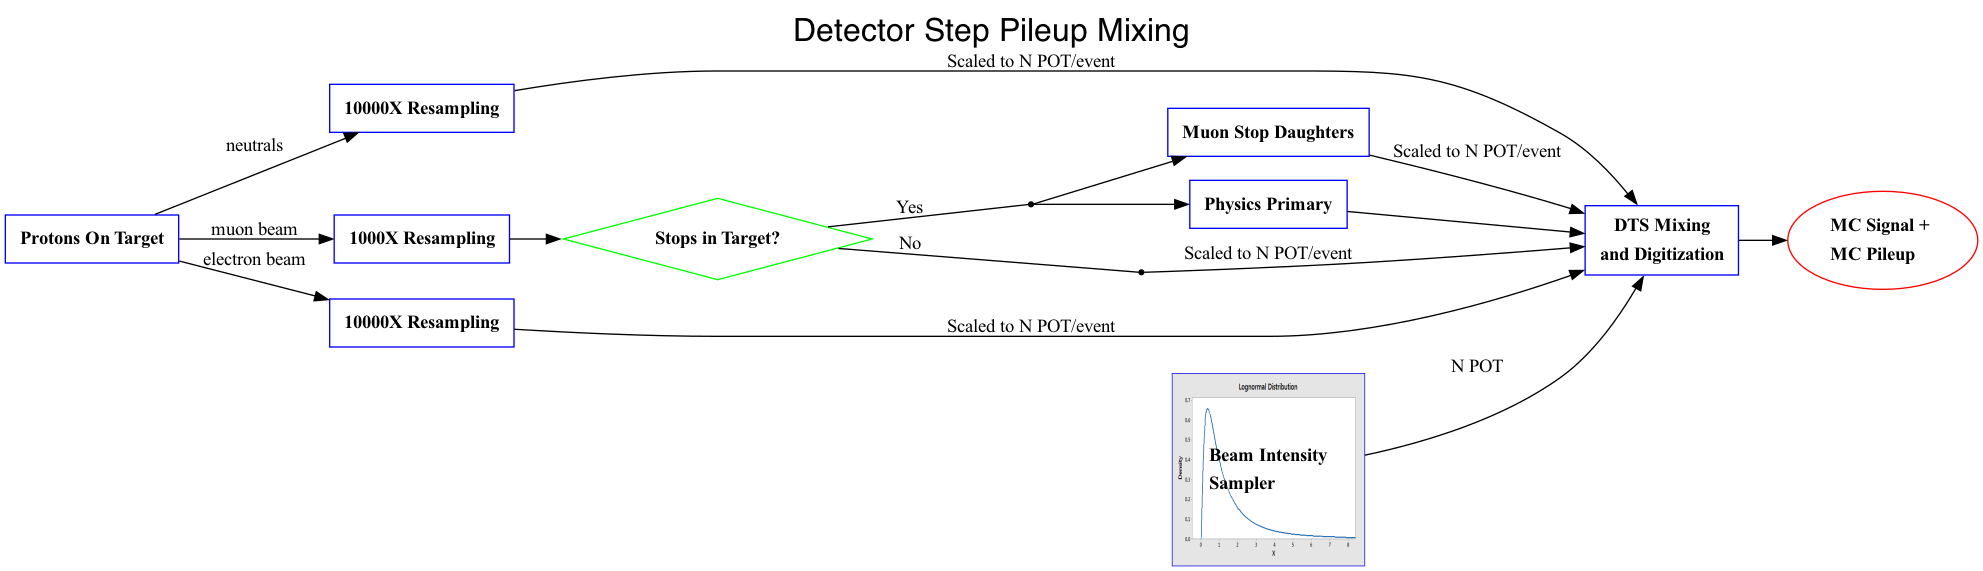
\includegraphics[width=\textwidth]{figures/DTS_Mixing.png}%
\caption{Workflow for producing simulated signal events with overlaid simulated beam pileup.}
\label{fig:dts_mixing}
\end{figure}

\begin{figure}[ht!]
\centering
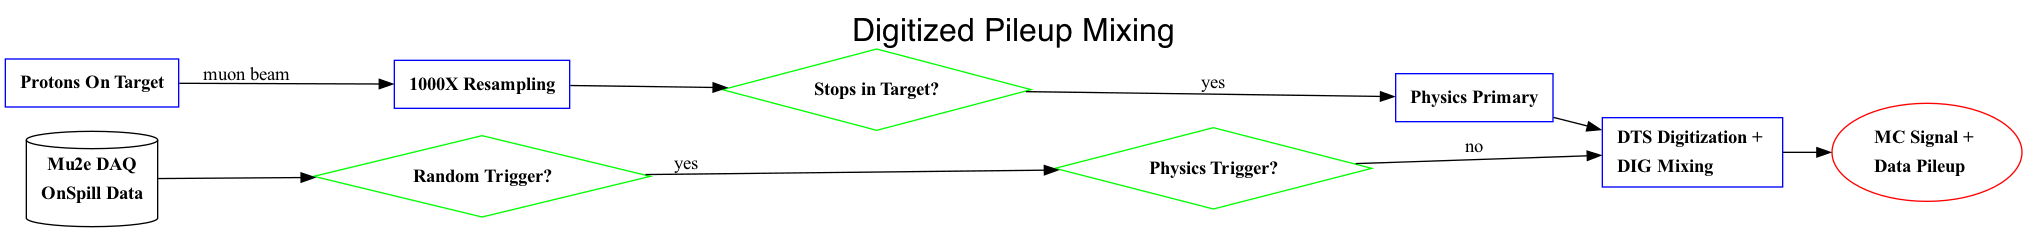
\includegraphics[width=\textwidth]{figures/DIG_Mixing.png}%
\caption{Workflow for producing simulated signal events with overlaid beam pileup extracted from data.}
\label{fig:dig_mixing}
\end{figure}

\subsection{Geant4 Physics processes}
The main physics interactions are simulated using a modification of the GEANT4 "Shielding" physics list. The main modification consists of increasing the threshold used to pass from the Bertini Cascade (BERT) model for low energy hadron-nucleus interactions to the Fritiof (FTF) model from 4-5 GeV to 9.5-9.9 GeV to better reproduce the experimental data on pion production. Nuclear de-excitations and radioactive decay of long-lived isotopes are included. Hyperon and anti-baryon production is obtained from the chiral invariant phase space model (CHIPS). Neutron simulation uses the high precision model (HP) up to 20 MeV. This is particularly relevant for the prediction of the thermal neutron background.

Geant4 is used only to produce the electrons and the photons from the atomic cascade to the ground state for muon capture in the aluminum stopping target. The nuclear muon capture, the muon decay in orbit, the radiative muon capture, and the muon conversion are simulated using custom generators (see below). The same holds for the radiative pion capture in the stopping target. Simulation of muon and pion captures outside of the stopping target is generally managed by Geant4, but custom generators have been created for particular studies related to detector calibration.  

Additional Monte Carlo codes are used to validate and evaluate systematic uncertainties in the predictions of critical quantities obtained with Geant4. MARS has been extensively used to study the radiation levels in the Mu2e hall, the effectiveness of the concrete shielding and of the Heat and Radiation Shield, and the dose and neutron fluence in the tracker and calorimeter electronics. The effect of concrete shielding on neutron and kaon radiation has also been studied with FLUKA and MCNP. Pion production in the PT has been investigated with MARS, MCNP, FLUKA, and PHITS, while Geant4 expectation for antiproton production in the production target has been corrected given its disagreement with MARS, MCNP, and FLUKA~\cite{Mu2e:2022ggl}. 

\subsection{Geometry description}
The experimental hall as designed for the first run of the experiment is shown in Fig.~\ref{fig:mu2e_geom}. The main information obtained from the simulation of the passive parts is the effectiveness of the shielding against the radiation produced by beam interactions and cosmic rays. The simulation includes the dirt surrounding the detector hall, the building walls, the concrete shielding blocks, the solenoids warm and cold mass, the radiation shield, the mechanical structure of the tracker and calorimeter, the beam dump downstream of the proton beam with the extinction monitor, ... The amount, type, and location of shielding have been decided as a compromise between budget considerations and the amount of radiation acceptable for the different sub-systems. It will be reviewed for Run II according to the result of Run I.
 
The geometrical description of each sub-system is maintained by the corresponding working groups. The level of detail of the geometry description is a compromise between the time needed to simulate the events and the agreement between data and Monte Carlo simulation. The main parameters (e.g. material composition, number of elements, single element dimension, and location) are included in the geometry database. The dimensions and positions of the active parts (tracker straw tubes, Ecal crystals, ...) are the nominal ones: mechanical tolerances, gravitational sags, or misalignments are introduced at the digitization level.

A separate geometry package has been realized for the detector commissioning with cosmic rays. The simulation of the experimental setup in this {\em extracted position} includes the tracker and calorimeter out of the Detector Solenoid and a few modules of the Cosmic Ray Veto on top of them (Figure~\ref{fig:mu2e_geom}(right)). Alternative geometrical descriptions for the detector have been realized using MARS and FLUKA to determine the uncertainty of simulation estimates of the radiation levels and the stopped muon yield.

\begin{figure}[ht!]
\begin{center}
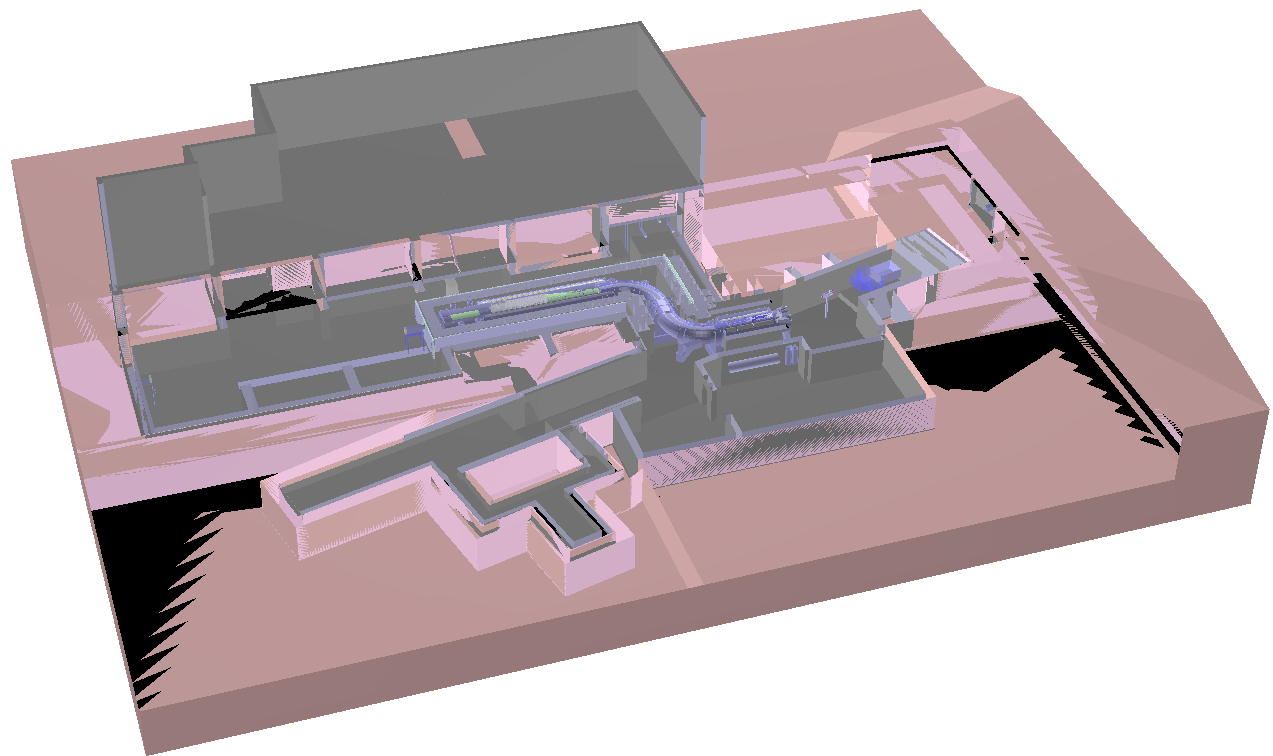
\includegraphics[height=0.29\linewidth]{figures/mu2eHall.png}
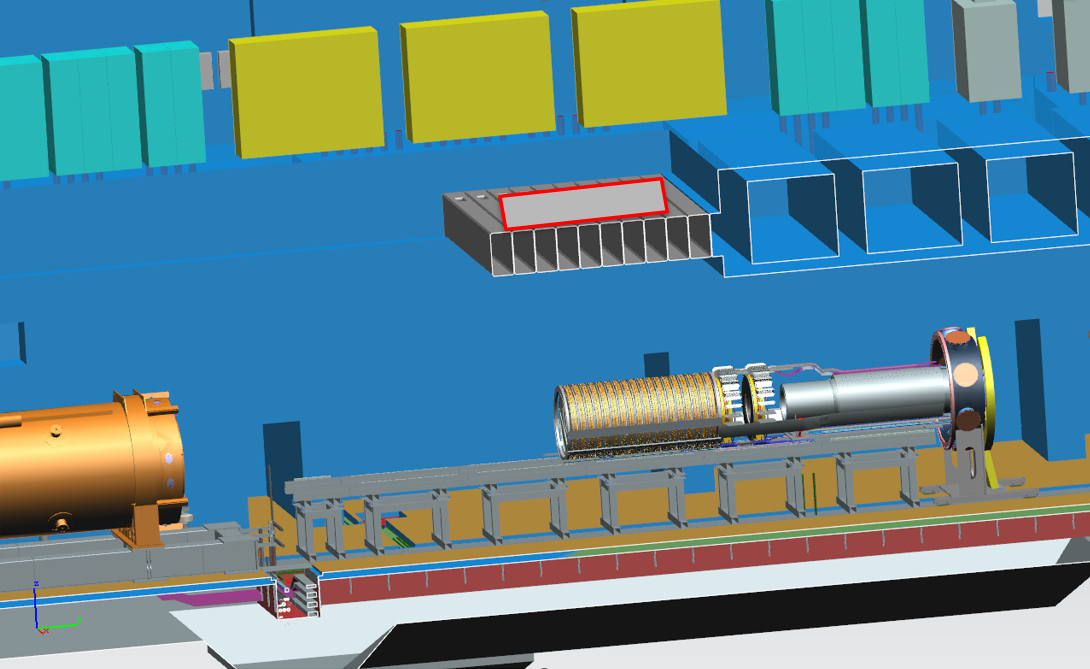
\includegraphics[height=0.29\linewidth]{figures/geom_extracted.png}
\caption{Left: the Mu2e experiment and building in the Geant4 Offline simulation. Right: Mu2e detectors in the extracted position.}
\label{fig:mu2e_geom}
\end{center}
\end{figure}

%Each sub-system group has developed the geometry description of the setup used for beam or cosmic ray tests of the prototypes or for the Vertical Slice Test of the first production modules. Although these are in general standalone programs, they have been an important tool to validate the detector description in the Offline repository. 

\subsection{Magnetic field maps}
Detailed magnetic field maps are produced using the OPERA 3D~\cite{opera3D} and HELICALC~\cite{helicalc} software packages using (warm) as-measured conductor geometries and coil positions provided by the Mu2e project solenoid construction team. The field is stored as a discrete vector map over a Cartesian grid, separately for the Production Solenoid (PS), Transport Solenoid (TS), Detector Solenoid (DS), and the region outside all the solenoids. The effect of re-bar in the concrete shielding has been calculated but not yet included. Field maps for special run conditions used for calibration purposes have also been generated. The field map is accessed through a software interface that dynamically interpolates the field vectors from the 9 grid points nearest the requested reference point.

The Mu2e operations team will determine the in-situ DS magnetic field using a custom survey device that will measure the magnetic field components at fixed locations within a cylindrical coordinate grid. A fit to the measured data using a combination of a multi-pole expansion and relaxation ANN constrained to Maxwell's equations will be used to interpolate and average the measurements into the Cartesian grid format. This map will be corrected for the estimated effect of re-bar in shielding materials that can't be in place during the field survey.

Publication quality simulations and reconstruction will use the field map determined from the survey. Changes in physics objects reconstructed using alternative maps spanning the measurement and shielding magnetization uncertainties will be used to estimate the systematic errors on physics measurements due to residual field map uncertainties.


\subsection{Detector response}
Each sub-system has a dedicated simulation of its digitization. This includes a parameterization of the physics processes bringing the signal from the position where the energy is deposited to the readout electronics and also the simulation of the electronics response. Simulated digitization uses the timing information from the (simulated) DAQ clock system used to define the start and stop of each digitization period, including the 5-fold repeating pattern of different event start times and lengths caused by the period mis-match of the booster and the delivery ring clocks.
%\red {So we foresee to use some database information during digitization?}

\begin{itemize}
\item{Tracker -} energy deposits in the straw tubes from different particles are collated and processed by applying a parameterized simulation of the drift time, gas amplification, signal transit time along the wire, electronic amplification, and shaping. Electronic signals at the straw ends are superimposed and the resultant waveform is digitized. Only digitized hits passing the discrimination threshold at both ends are saved. 

\item{Calorimeter -} energy deposits in each crystal are grouped in time. The number of photons produced by scintillation takes into account the average light response uniformity measured during crystal qualification. The number of photo-electrons obtained using the average PDE of the SiPMs is smeared with a Poisson distribution. The digitizer waveforms corresponding to energy deposits in the same readout unit are superimposed. Radiation-induced noise and electronic noise are added. Zero suppression is reproduced.

\item{Cosmic Ray Veto -} energy deposits in each module are grouped in time. The bunch time structure is applied (only for the on-spill simulation). The time distribution of the charge collected by the SiPMs located at the edge of each module is calculated using the scintillator light yield, the WLS collection efficiency, the light attenuation along the fiber, the reflection probability on the walls, and the SiPM photon detection efficiency. The charge collected by the SiPMs is transformed into signal waveforms after applying a random time jitter and photo-electron fluctuation. ADC and TDC counts are obtained by applying waveform sampling and discrimination. 

\item{Stopping Target Monitor -} energy deposited by each photon in the HPGe detector is used to generate a waveform according to the deposited ionizing energy, measured gain, and collection efficiency. Waveforms from different photons are superimposed using the expected time and energy distribution. Electronic noise from the pre-amplifier and amplifier is added. The resulting waveforms are digitized using the 16bit ADC, and are used together to form STMWaveformDigis. A similar technique will be used for LaBr response.

\item{Extinction Monitor -} energy deposits are converted into electron-hole pairs. The number of charge carriers is fluctuated using the silicon Fano factor of 0.1. The deposited charge is split into a number of clusters uniformly distributed along the particle path inside the sensor. Each cluster is drifted individually. The sum of the charge reaching the pre-amplifier with its time structure is passed to a discriminator that simulates the time and time over threshold response of the readout chip. At the final stage, the digitization algorithm adds random hits to the output~\cite{ExtMon:2014}.
\end{itemize}


\subsection{Simulation campaigns}
Several simulation campaigns have been conducted since the inception of the experiment to guide the design and evaluate the corresponding physics performance. The SU2020 campaign was based on workflows developed in 2018, and the output was used to update the sensitivity estimate of the experiment for expected run 1 operations. That work pulled in effort from a number of younger collaborators, and was published \cite{Mu2e:2022ggl}.  The most recent campaign, MDC2020, used updated geometries, detector response simulations, and a streamlined workflow to generate
large samples of beam, pileup, signals, and physics backgrounds. The principal output of MDC2020 was a large sample of conversion signals with pileup, used in algorithm development, plus pure pileup events, for trigger studies.
MDC2020 used the Production Operations Management Service (POMS) to run complex grid campaigns, and GitHub to store scripts and configuration files. The whole effort was driven by the Mu2e Production Manager. 
Different sets of calibration and alignment conditions were simulated to evaluate their impact on the reconstruction efficiency. Most of the conditions were also directly extracted directly from the database, providing a test of the condition system in a production setting. These data have proved essential to improve and evaluate the performance of reconstruction algorithms, including those used in the trigger, and perform the SU2020 sensitivity study~\cite{Mu2e:2022ggl}. 

\subsection{Ensembles}
\label{subsec:ensembles}
While useful for software development and some physics studies, individual background streams produced in MDC2020 are not representative of the mixed-signal samples that will be used for analysis. Mock Data samples were introduced to provide a more accurate model of what Mu2e will record during data-taking phases. These samples are produced by merging individual background sources (Pile-up, cosmic rays, DIO, RPC, ...) into a data collection with mixed content, according to event event fractions expected in real data. The combined sample is then passed through our digitization and reconstruction framework to create "data-like" samples. Ensemble creation uses a dedicated art input module that knows how to sample multiple input files. In addition to the development of calibration procedures and analysis frameworks, the ensemble data sets will also enable test of the computing infrastructure in more realistic conditions. Production of large ensemble data sets for dry-run tests of the offline calibration and processing workflow at scale is foreseen before the start of Mu2e beam running.